\chapter{Introducción al teorema de la función implícita}
\section{Funciones implícitas}
Cuando iniciamos como estudiantes de cálculo, usualmente una función es dada por una expresión analítica como:
$$f(x)=\sqrt{x^2+1}$$
$$h(t)=\cos(5t)$$
$$g(y)=y^3+6$$
De hecho, hace 250 años este fue el enfoque adoptado por Leonard Euler (1707-1783) cuando escribió: "Una función de una cantidad variable es una expresión analítica compuesta"
\\Casi inmediatamente, uno encuentra que la noción de "función dada por una fórmula" esta es demasiado limitado para los fines del cálculo.\\En contraste a la usual definición que se suele dar, una definición más precisa de \textit{función f con dominio X y rango Y} es la que sigue.
\begin{Def}
Una función con dominio X y rango Y es un subconjunto del producto cartesiano $X\times Y$ que cumple las siguientes propiedades:
\begin{enumerate}
    \item  Para cada $x\in X$ existe un elemento $(x,y)\in f$
    \item Si $(x,y)\in f$ y $(x,\tilde{y})\in f$, entonces $y=\tilde{y}$
\end{enumerate}
\end{Def} 
Por ejemplo, la siguiente expresión define un subconjunto de $\R^2$ descrita en la figura \ref{Figura1_1}\\
\begin{equation}
    y^5+16y-32x^3+32x=0
    \label{ecuacion1}
\end{equation}
\begin{figure}[htb]
\begin{center}
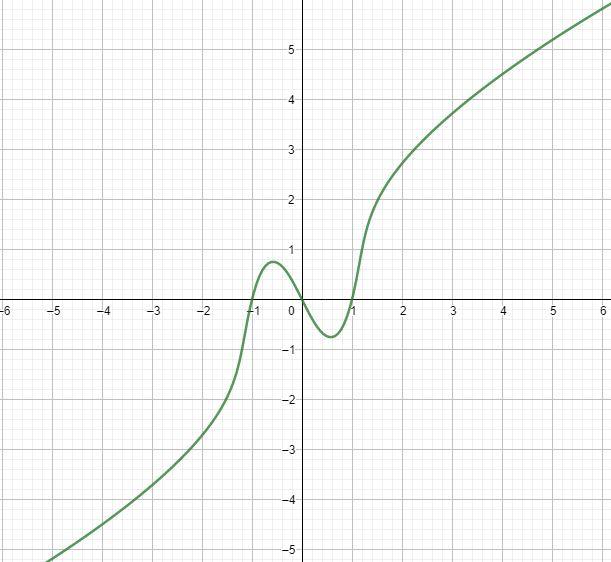
\includegraphics[width=8.5cm]{figura1_1.jpg}
\label{Figura1_1}
\caption{Gráfica de puntos que satisfacen \ref{ecuacion}}
\vspace*{0.05in}
\end{center}
\end{figure}
La gráfica nos muestra que aunque no se defina una fórmula explícitamente, con la definición previa el subconjunto $$f=\{(x,y)\in X\times Y: y^5+16y-32x^3+32x=0\}$$ es efectivamente una función. \\A este tipo de funciones las llamaremos \textit{funciones implícitas} y son ellas en las cuales nos centraremos en el desarrollo de este ensayo.